% !TeX root = mainstarkov.tex
% !TeX program = xelatex
% !TeX encoding = UTF-8
\section{Технический проект}

\subsection{Общая характеристика организации решения задачи}

Разрабатываемый модуль динамической маршрутизации является алгоритмическим ядром системы IndoorNav и обеспечивает построение оптимальных маршрутов внутри здания с учётом динамически изменяющихся препятствий. Модуль не зависит от пользовательского интерфейса и может использоваться как в мобильном приложении, так и в серверных компонентах.

Архитектура модуля следует принципу разделения ответственности: структуры данных графа выделены в отдельные классы (\texttt{NavNode}, \texttt{NavEdge}, \texttt{NavGraph}), алгоритмы поиска пути инкапсулированы в методах класса \texttt{NavGraph}, а специфичная логика эвакуации вынесена в сервис \texttt{EmergencyService}. Такое разделение упрощает тестирование: алгоритм Дейкстры можно проверять независимо от логики ЧС, а структуры данных -- независимо от алгоритмов. Разделение ответственности между классами опирается на типовые приёмы объектно-ориентированного проектирования \cite{gof,freeman} и принципы чистой архитектуры \cite{fowler}.

Система построена по архитектурному шаблону MVVM \cite{mauimvvm,albahari} и разделена на четыре слоя: слой представления (View), слой моделей представления (ViewModel), сервисный слой (Service) и слой моделей данных (Model); ниже располагается хранилище данных в формате JSON. Схема архитектуры программной системы с указанием состава компонентов и связей между слоями приведена на рисунке~\ref{arch:image}. Компоненты, реализующие динамическую маршрутизацию (\texttt{MainViewModel}, \texttt{NavGraphService}, \texttt{EmergencyService}, \texttt{NavGraph}, \texttt{NavNode}, \texttt{NavEdge}, \texttt{RouteStep}), выделены на схеме цветом.

\begin{figure}[H]
\centering
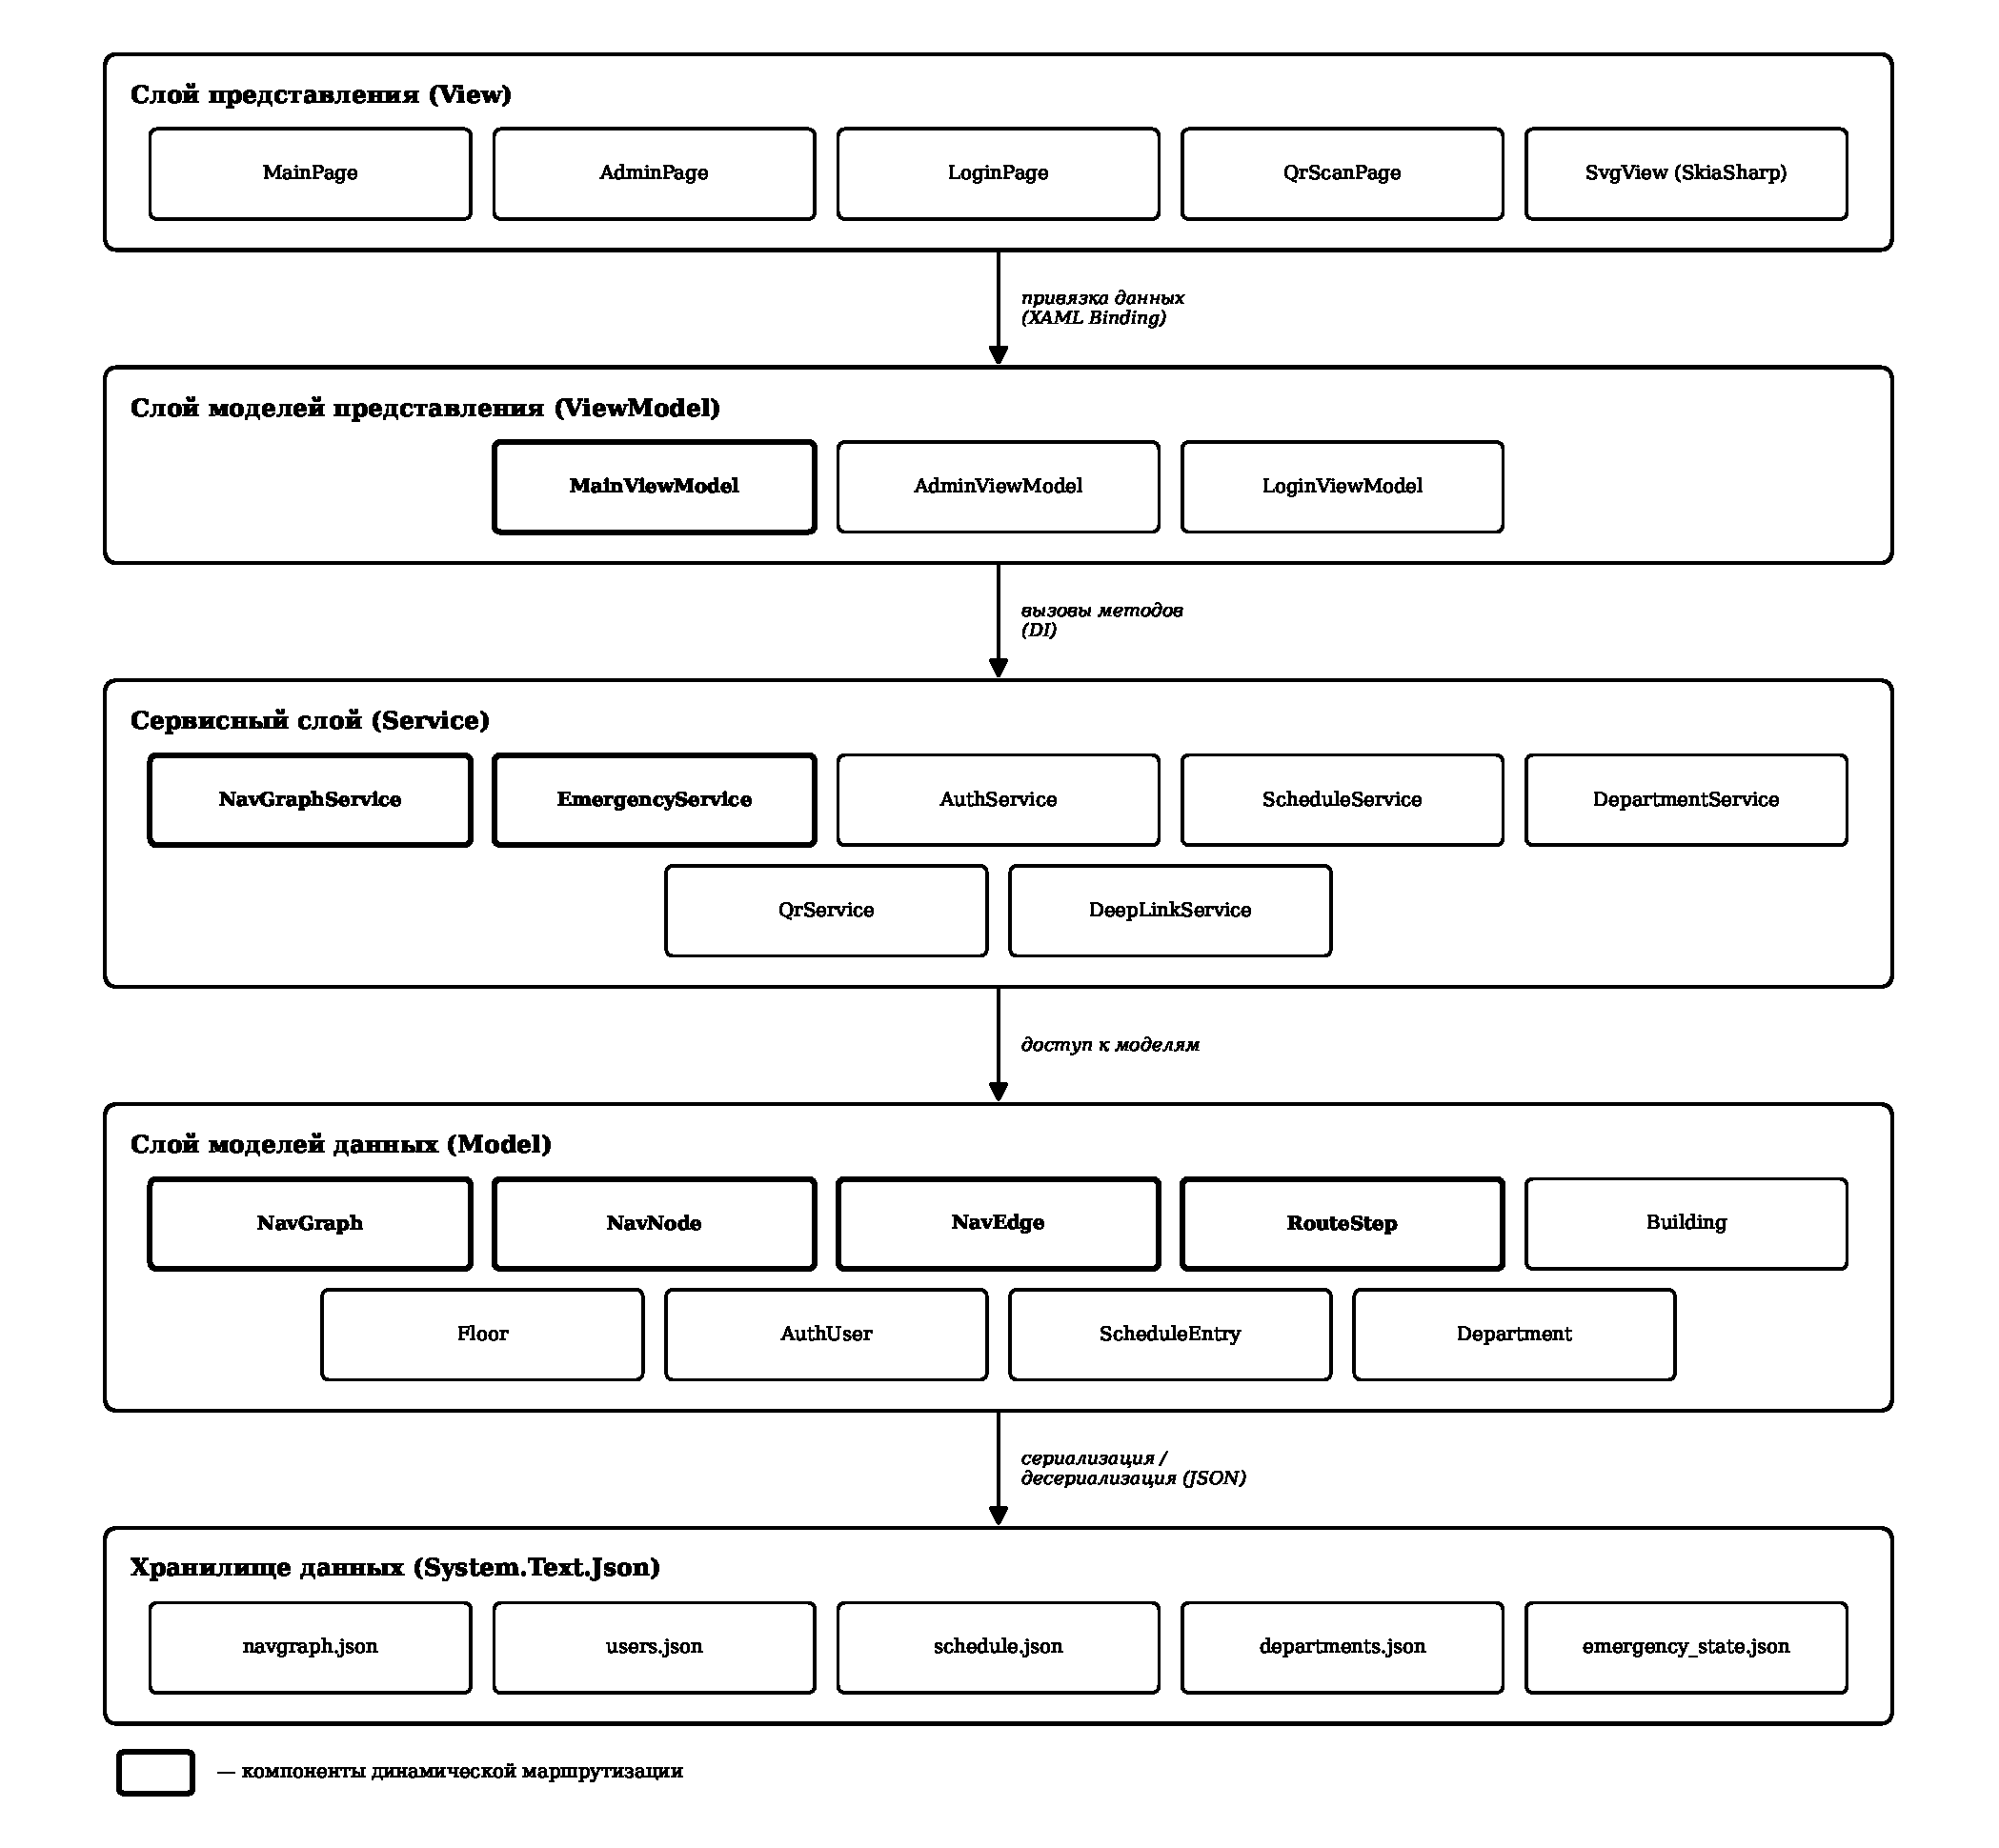
\includegraphics[width=\textwidth]{Pictures/arch.eps}
\caption{Схема архитектуры программной системы IndoorNav}
\label{arch:image}
\end{figure}

Каждый слой зависит только от нижележащего: представление взаимодействует с моделями представления через механизм привязки данных XAML \cite{xaml}, модели представления вызывают методы сервисов через внедрение зависимостей (DI), сервисы оперируют моделями данных, а сохранение и загрузка графа, пользователей, расписания и состояния ЧС выполняются сериализацией моделей в JSON средствами \texttt{System.Text.Json}. Такая слоистая организация изолирует алгоритмическое ядро от пользовательского интерфейса и платформенных особенностей \cite{yarovaya2022,marinin2024}.

Главная особенность решения -- поддержка динамического исключения узлов без модификации исходного графа. Это позволяет системе перестраивать маршруты в реальном времени при блокировке проходов, не перезагружая данные и не создавая копии графа. Исключённые узлы передаются как параметр алгоритма и проверяются при обходе рёбер.

\subsection{Обоснование выбора технологий реализации}

\subsubsection{Язык C\# и платформа .NET.}

Реализация выполнена на языке C\# \cite{richter} в рамках платформы .NET MAUI \cite{maui}, что обеспечивает единый код для Android, iOS и Windows. Кроссплатформенный подход выбран вместо нативной разработки под каждую ОС: он сохраняет единую кодовую базу, что подтверждается опытом перехода от Xamarin к .NET MAUI \cite{ershov2021,ilichev2018} и сравнительными исследованиями кроссплатформенных мобильных технологий \cite{zhukovskaya2017,eskendir2019,feshina2022,jia2018}. C\# предоставляет строгую типизацию для моделирования навигационного графа, обобщённые коллекции (\texttt{Dictionary}, \texttt{SortedSet}, \texttt{HashSet}) для эффективной реализации алгоритмов и LINQ для фильтрации узлов по зданию, этажу и типу.

\subsubsection{Стандартные коллекции .NET.} 

Для реализации алгоритма Дейкстры используются стандартные коллекции .NET без привлечения сторонних библиотек: \texttt{SortedSet<(float, string)>} для очереди с приоритетом, \texttt{Dictionary<string, float>} для расстояний, \texttt{Dictionary<string, string?>} для предшественников, \texttt{HashSet<string>} для исключённых узлов. Это обеспечивает отсутствие внешних зависимостей и простоту отладки.

\subsubsection{Сериализация System.Text.Json.} 

Загрузка и сохранение навигационного графа выполняется с использованием \texttt{System.Text.Json} \cite{systemtextjson} с настройкой \texttt{WriteIndented = true}. Формат JSON \cite{json} выбран как компактный, читаемый и поддерживаемый на всех целевых платформах; среди форматов хранения текстовых данных он даёт хороший баланс между размером и удобством обработки \cite{naumov2021}.

\subsection{Архитектура алгоритмического ядра}

Модуль маршрутизации состоит из следующих компонентов:
\begin{itemize}
\item \textbf{NavNode} -- класс узла графа с атрибутами (координаты, этаж, тип, флаги);
\item \textbf{NavEdge} -- класс ребра графа (связь между узлами с весом);
\item \textbf{NavGraph} -- класс графа, хранящий узлы и рёбра, предоставляющий методы поиска пути;
\item \textbf{EmergencyService} -- сервис поиска ближайшего эвакуационного выхода;
\item \textbf{NavGraphService} -- сервис загрузки, сохранения и предоставления графа.
\end{itemize}

Все компоненты регистрируются в контейнере внедрения зависимостей (\texttt{MauiProgram.cs}) как singleton \cite{mauidi}, что обеспечивает единый экземпляр на всё время работы приложения и согласованность состояния. Внедрение зависимостей снижает связанность модулей и упрощает их раздельное тестирование \cite{sazonov2024,uvarov2016}.

Схема взаимодействия слоёв MVVM с выделением алгоритмического модуля приведена на рисунке~\ref{starkovmvvm:image}.

\begin{figure}[H]
\centering
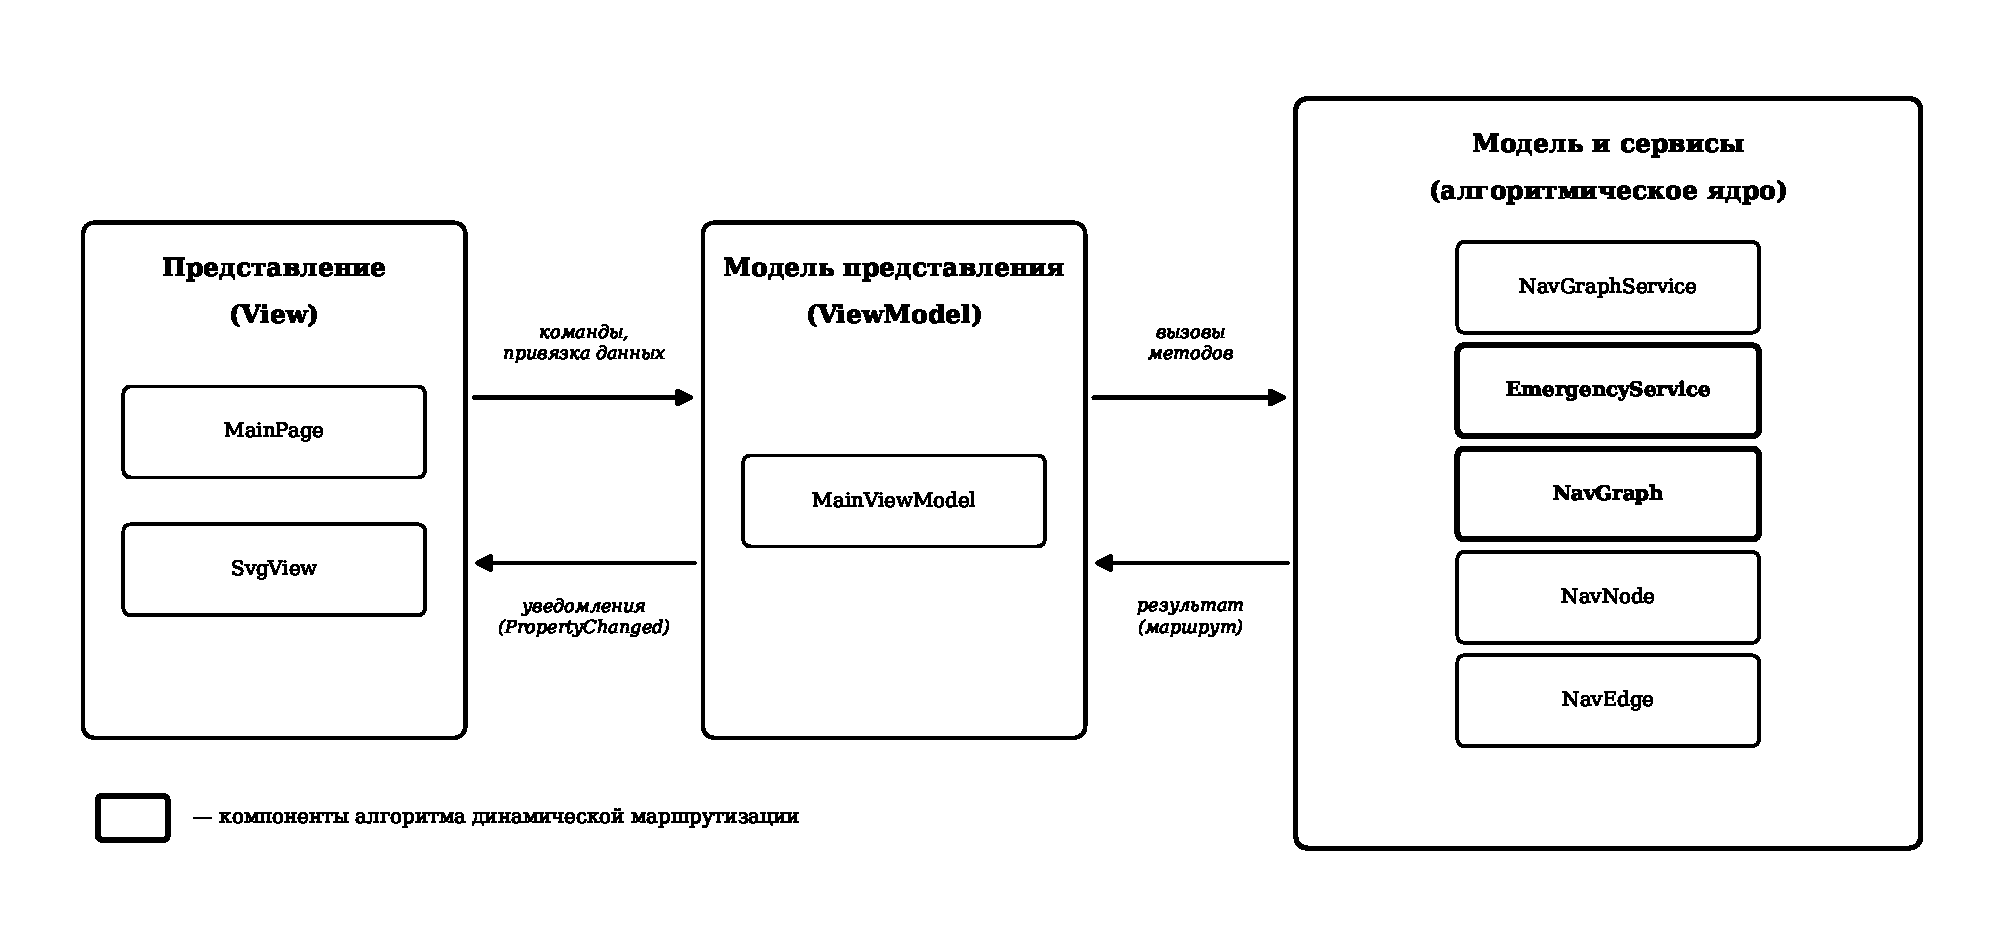
\includegraphics[width=0.95\textwidth]{Pictures/starkovmvvm.eps}
\caption{MVVM-архитектура приложения с выделением алгоритмического модуля}
\label{starkovmvvm:image}
\end{figure}

\subsection{Структуры данных навигационного графа}

\subsubsection{Класс NavNode.} 

Узел графа представляет точку на плане этажа (помещение, коридор, перекрёсток, лестничная площадка, выход) и содержит следующие свойства:
\begin{itemize}
\item \texttt{Id} -- уникальный идентификатор узла (string);
\item \texttt{Name} -- отображаемое название для пользователя (string);
\item \texttt{X}, \texttt{Y} -- координаты на плане этажа в условных единицах (float);
\item \texttt{FloorNumber} -- номер этажа (int), используется для определения межэтажных переходов;
\item \texttt{BuildingId} -- идентификатор здания/корпуса (string);
\item \texttt{IsTransition} -- флаг узла перехода между этажами;
\item \texttt{IsElevator} -- флаг лифтового узла;
\item \texttt{IsExit} -- флаг основного выхода;
\item \texttt{IsEvacuationExit} -- флаг эвакуационного выхода;
\item \texttt{IsFireExtinguisher} -- флаг огнетушителя (отображается при ЧС);
\item \texttt{IsQrAnchor} -- флаг QR-якоря для позиционирования;
\item \texttt{IsRoom} -- флаг узла-аудитории;
\item \texttt{IsWaypoint} -- флаг путевой точки;
\item \texttt{IsHidden} -- флаг скрытого узла (не отображается на карте);
\item \texttt{TransitionGroupId} -- идентификатор группы перехода для связывания узлов на разных этажах;
\item \texttt{RoomId} -- необязательный идентификатор помещения из внешней системы.
\end{itemize}

Узлы с флагами \texttt{IsExit} и \texttt{IsEvacuationExit} используются как целевые точки при построении эвакуационного маршрута.

\subsubsection{Класс NavEdge.} 

Ребро графа представляет проход между двумя точками и содержит:
\begin{itemize}
\item \texttt{FromId}, \texttt{ToId} -- идентификаторы соединяемых узлов;
\item \texttt{Weight} -- вес ребра, вычисляемый как расстояние между узлами с учётом типа прохода;
\item \texttt{IsCrossFloor} -- флаг межэтажного перехода.
\end{itemize}

Вес ребра вычисляется автоматически при создании: для узлов на одном этаже $w = \sqrt{(x_2 - x_1)^2 + (y_2 - y_1)^2}$, для узлов на разных этажах $w = 150$.

Фиксированный штраф 150 для межэтажных переходов отражает повышенные затраты времени на подъём/спуск по лестнице или лифту. Граф является неориентированным: при добавлении ребра создаются две направленные записи (от A к B и от B к A) с одинаковым весом.

\subsubsection{Класс NavGraph.} 

Граф хранит коллекции узлов и рёбер и предоставляет алгоритмы поиска пути:

\begin{itemize}
\item \texttt{Nodes} -- список всех узлов графа (\texttt{List<NavNode>});
\item \texttt{Edges} -- список всех рёбер графа (\texttt{List<NavEdge>});
\item \texttt{GetNode(id)} -- быстрый доступ к узлу по идентификатору через внутренний словарь;
\item \texttt{FindPath(startId, endId, excludeIds)} -- поиск кратчайшего пути методом Дейкстры;
\item \texttt{BuildAdjacency()} -- построение списка смежности для оптимизации поиска.
\end{itemize}

Метод \texttt{BuildAdjacency()} строит словарь связей \texttt{Dictionary<string, List<(string neighbor, float weight)>>}, который используется алгоритмом Дейкстры для быстрого доступа к соседям каждой вершины. Построение выполняется один раз при загрузке графа.

Пример навигационного графа здания приведён на рисунке~\ref{navgraph:image}. Узлы обозначены кружками с идентификаторами, рёбра -- линиями с указанием веса. Узлы-выходы выделены двойной рамкой, узлы переходов между этажами -- штриховой рамкой.

\begin{figure}[H]
\centering
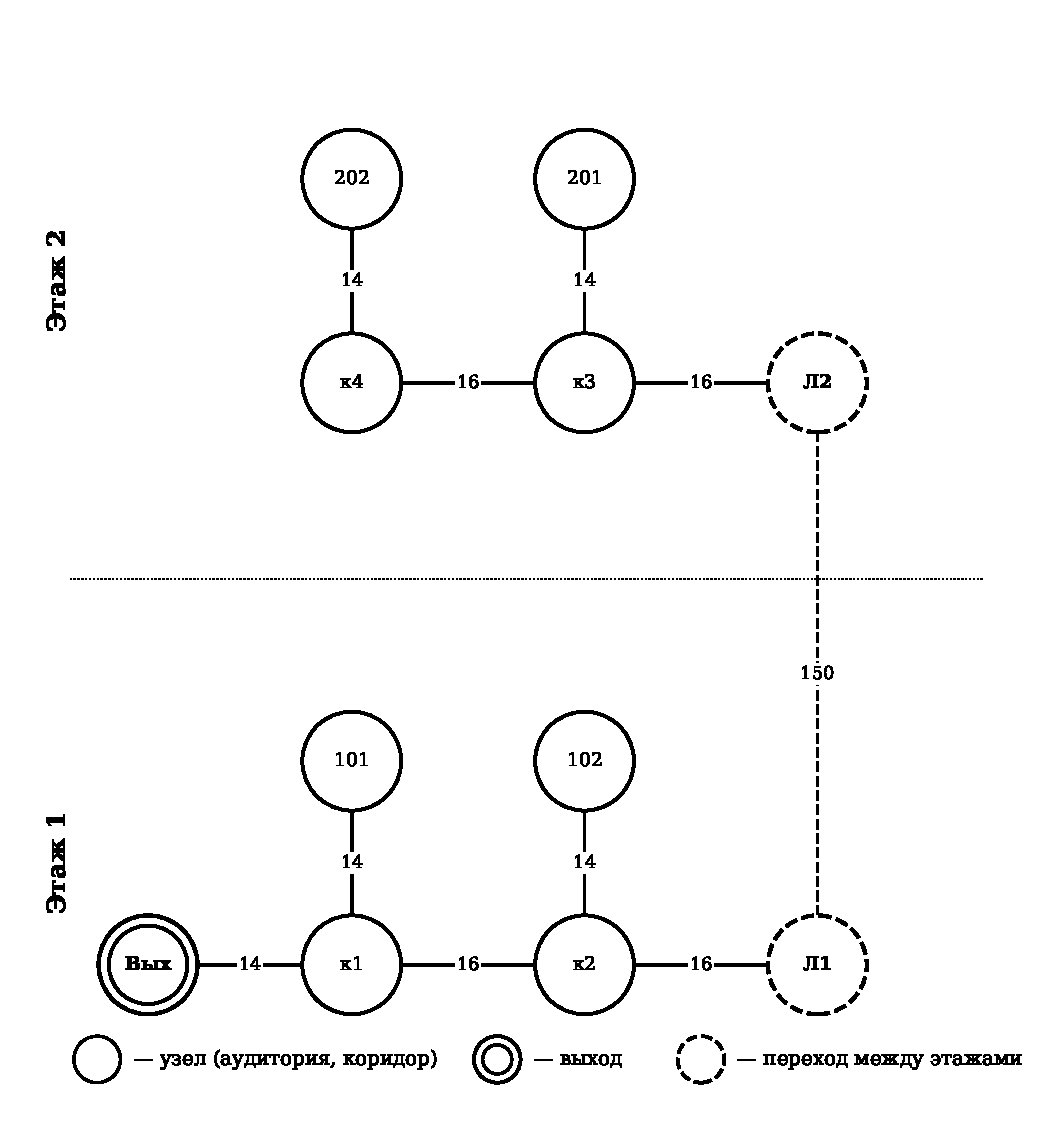
\includegraphics[width=0.85\textwidth]{Pictures/graf.eps}
\caption{Пример структуры навигационного графа здания}
\label{navgraph:image}
\end{figure}

\subsection{Проектирование хранения данных}

Все данные приложения хранятся локально, в текстовых файлах формата JSON~-- так навигация не зависит от сети, а файлы при необходимости легко просмотреть и поправить вручную. Чтение и запись идут через \texttt{System.Text.Json}: объекты модели преобразуются в формат JSON и обратно без использования промежуточного слоя базы данных \cite{vinnikov2022}. Данный подход оправдан для навигационного графа здания, поскольку граф полностью размещается в оперативной памяти, а его модификация происходит редко — преимущественно при разметке карты администратором.

Перечень файлов данных и их назначение приведены в таблице~\ref{datafiles:table}.

\begin{xltabular}{\textwidth}{|l|X|}
	\caption{Файлы данных приложения\label{datafiles:table}}\\ \hline
	\centrow Файл & \centrow Содержимое \\ \hline
	\thead{1} & \centrow 2 \\ \hline
	\endfirsthead
	\continuecaption{Продолжение таблицы \ref{datafiles:table}}
	\centrow Файл & \centrow Содержимое \\ \hline
	\finishhead
	\texttt{navgraph.json} & Навигационный граф: массивы узлов и рёбер \\ \hline
	\texttt{users.json} & Учётные записи с хешами паролей и ролями \\ \hline
	\texttt{departments.json} & Кафедры и учебные группы \\ \hline
	\texttt{schedule.json} & Расписание занятий по аудиториям и группам \\ \hline
	\texttt{emergency\_state.json} & Список зданий, где включён режим ЧС
\end{xltabular}

Главный для маршрутизации файл~-- \texttt{navgraph.json}. На верхнем уровне это объект с двумя массивами: \texttt{Nodes} (узлы) и \texttt{Edges} (рёбра). Каждый узел хранит идентификатор, координаты, этаж, корпус и набор флагов типа; каждое ребро~-- идентификаторы концов, длина и признак межэтажного перехода. Структура напрямую повторяет классы \texttt{NavNode} и \texttt{NavEdge}, поэтому отдельная схема преобразования не нужна. Фрагмент файла с одним узлом и одним ребром выглядит так:

\newpage
\begin{figure}[H] 
\begin{lstlisting}
{
	"Nodes": [
	{ "Id": "a-101", "Name": "101", "X": 320.5, "Y": 148.0,
		"FloorNumber": 1, "BuildingId": "A",
		"IsRoom": true, "IsExit": false, "IsEvacuationExit": false }
	],
	"Edges": [
	{ "FromId": "a-101", "ToId": "a-kor1", "Weight": 42.3,
		"IsCrossFloor": false }
	]
}
\end{lstlisting}
\end{figure}

При запуске \texttt{NavGraphService} читает файл в объект \texttt{NavGraph}, после чего граф готов к работе. Сохранение выполняется обратной операцией с отступами (\texttt{WriteIndented}), чтобы файл оставался читаемым.

\subsection{Проектирование алгоритмов маршрутизации}

Алгоритмы маршрутизации включают четыре компонента: построение кратчайшего маршрута по алгоритму Дейкстры, поиск ближайшего эвакуационного выхода, формирование пошаговых инструкций и определение множества заблокированных узлов.

\subsubsection{Реализация алгоритма Дейкстры}

Реализация алгоритма Дейкстры в методе \texttt{NavGraph.FindPath(startId, endId, excludeIds)} использует следующие структуры данных:
\begin{itemize}
\item \texttt{SortedSet<(float dist, string id)>} -- очередь с приоритетом для выбора вершины с минимальным расстоянием;
\item \texttt{Dictionary<string, float>} -- словарь текущих кратчайших расстояний от стартовой вершины;
\item \texttt{Dictionary<string, string?>} -- словарь предшественников для восстановления пути;
\item \texttt{ISet<string>?} -- множество исключаемых узлов (может быть null).
\end{itemize}.

\textbf{Динамическое исключение узлов.} Множество исключаемых узлов передаётся как параметр \texttt{excludeIds} и проверяется при рассмотрении соседей. Это позволяет исключать узлы без модификации графа. Конечный узел маршрута никогда не исключается, даже если его идентификатор присутствует в множестве.

\textbf{Обработка отсутствия пути.} Если после завершения алгоритма расстояние до целевой вершины остаётся равным \texttt{float.MaxValue} (вершина недостижима), метод возвращает пустой список. Это обеспечивает устойчивость системы: при полной блокировке пути приложение корректно информирует пользователя.

\textbf{Оптимизация списка смежности.} Перед запуском алгоритма строится словарь смежности \texttt{adj}, группирующий рёбра по исходящему узлу. Это позволяет получить всех соседей вершины за $O(1)$ вместо линейного поиска по списку рёбер.

\textbf{Обработка устаревших записей очереди.} При обновлении расстояния до вершины старая запись не удаляется из \texttt{SortedSet}, а проверяется при извлечении: если извлечённое расстояние превышает текущее, запись игнорируется. Это упрощает реализацию и избавляет от необходимости сложного обновления приоритетов.

\subsubsection{Алгоритм поиска ближайшего эвакуационного выхода}

Для режима чрезвычайной ситуации реализован алгоритм в методе \texttt{EmergencyService.FindNearestExitRoute(start, graph, excludeIds)}, который находит кратчайший путь до ближайшего эвакуационного выхода. Пример: 

\begin{figure}[H] 
\begin{lstlisting}
function FindNearestExitRoute(start, graph, excludeIds):

  exits = graph.Nodes.Where(n =>
    (n.IsExit or n.IsEvacuationExit)
    and n.BuildingId == start.BuildingId
    and excludeIds not contains n.Id)

  if exits is empty:
    exits = graph.Nodes.Where(n =>
      (n.IsExit or n.IsEvacuationExit)
      and excludeIds not contains n.Id)
  if exits is empty:
    return []

  dist[start.Id] = 0
  for each node in graph.Nodes:
    if node.Id != start.Id:
      dist[node.Id] = +infinity
    prev[node.Id] = null
  queue.Add((0, start.Id))
  adj = BuildAdjacency(graph)

  while queue is not empty:
    (d, uid) = queue.ExtractMin()
    if d > dist[uid]: continue
    for each (nid, w) in adj[uid]:
      if nid != start.Id and excludeIds contains nid:
        continue
      alt = d + w
      if alt < dist[nid]:
        queue.Remove((dist[nid], nid))
        dist[nid] = alt
        prev[nid] = uid
        queue.Add((alt, nid))

  bestExit = exits.OrderBy(e => dist[e.Id]).First()
  if bestExit == null or dist[bestExit.Id] == +infinity:
    return []

  path = []
  current = bestExit.Id
  while current != null:
    path.Add(nodeMap[current])
    current = prev[current]
  path.Reverse()
  return path
\end{lstlisting}
\end{figure}

\textbf{Интеграция с ViewModel.} При активации режима ЧС \texttt{MainViewModel} вызывает \texttt{ExecuteBuildEmergencyRoute()}, который определяет текущее положение пользователя (\texttt{StartNode}), формирует множество заблокированных узлов (\texttt{\_blockedNodeIds}), вызывает \texttt{EmergencyService.FindNearestExitRoute(start, graph, blocked)}, при наличии пути устанавливает конечный узел и вызывает \texttt{ExecuteBuildRoute()}, при отсутствии пути отображает сообщение <<Маршрут до выхода не найден>>.

\subsubsection{Механизм формирования пошаговых инструкций}

После построения маршрута \texttt{MainViewModel.BuildRouteSteps(path)} формирует пошаговые текстовые инструкции для пользователя. Метод группирует узлы маршрута по этажам в сегменты: для каждого сегмента определяется направление движения и формируется текст инструкции. Для межэтажных переходов добавляется шаг <<Перейдите на этаж N>> с указанием типа перехода (лестница/лифт). Каждому шагу назначается иконка (прямо, поворот, лестница, лифт, выход), определяется фокусный узел и прямоугольник для подсветки на карте. После формирования обновляются свойства интерфейса: \texttt{RouteSteps}, \texttt{CurrentStep}, \texttt{HasRoute}.

\subsubsection{Множество исключённых узлов}

Метод \texttt{MainViewModel.BuildExcludeSet(start, end)} формирует множество узлов, исключаемых из маршрута. В множество включаются все узлы с флагом \texttt{IsExit} или \texttt{IsEvacuationExit}, кроме стартового и конечного, а также все узлы, заблокированные пользователем (\texttt{\_blockedNodeIds}). Исключение выходов, не являющихся целевыми, предотвращает прохождение маршрута через другие выходы, что особенно важно в режиме эвакуации. Заблокированные узлы добавляются к множеству исключений, обеспечивая автоматическое перестроение маршрута в обход непроходимых участков.

\subsection{Процесс построения маршрута}

Описанные алгоритмы и структуры данных связываются в единый поток обработки запроса. Путь от действия пользователя до маршрута на экране проходит через все слои приложения и показан на рисунке~\ref{routeflow:image}.

\begin{figure}[H]
	\centering
	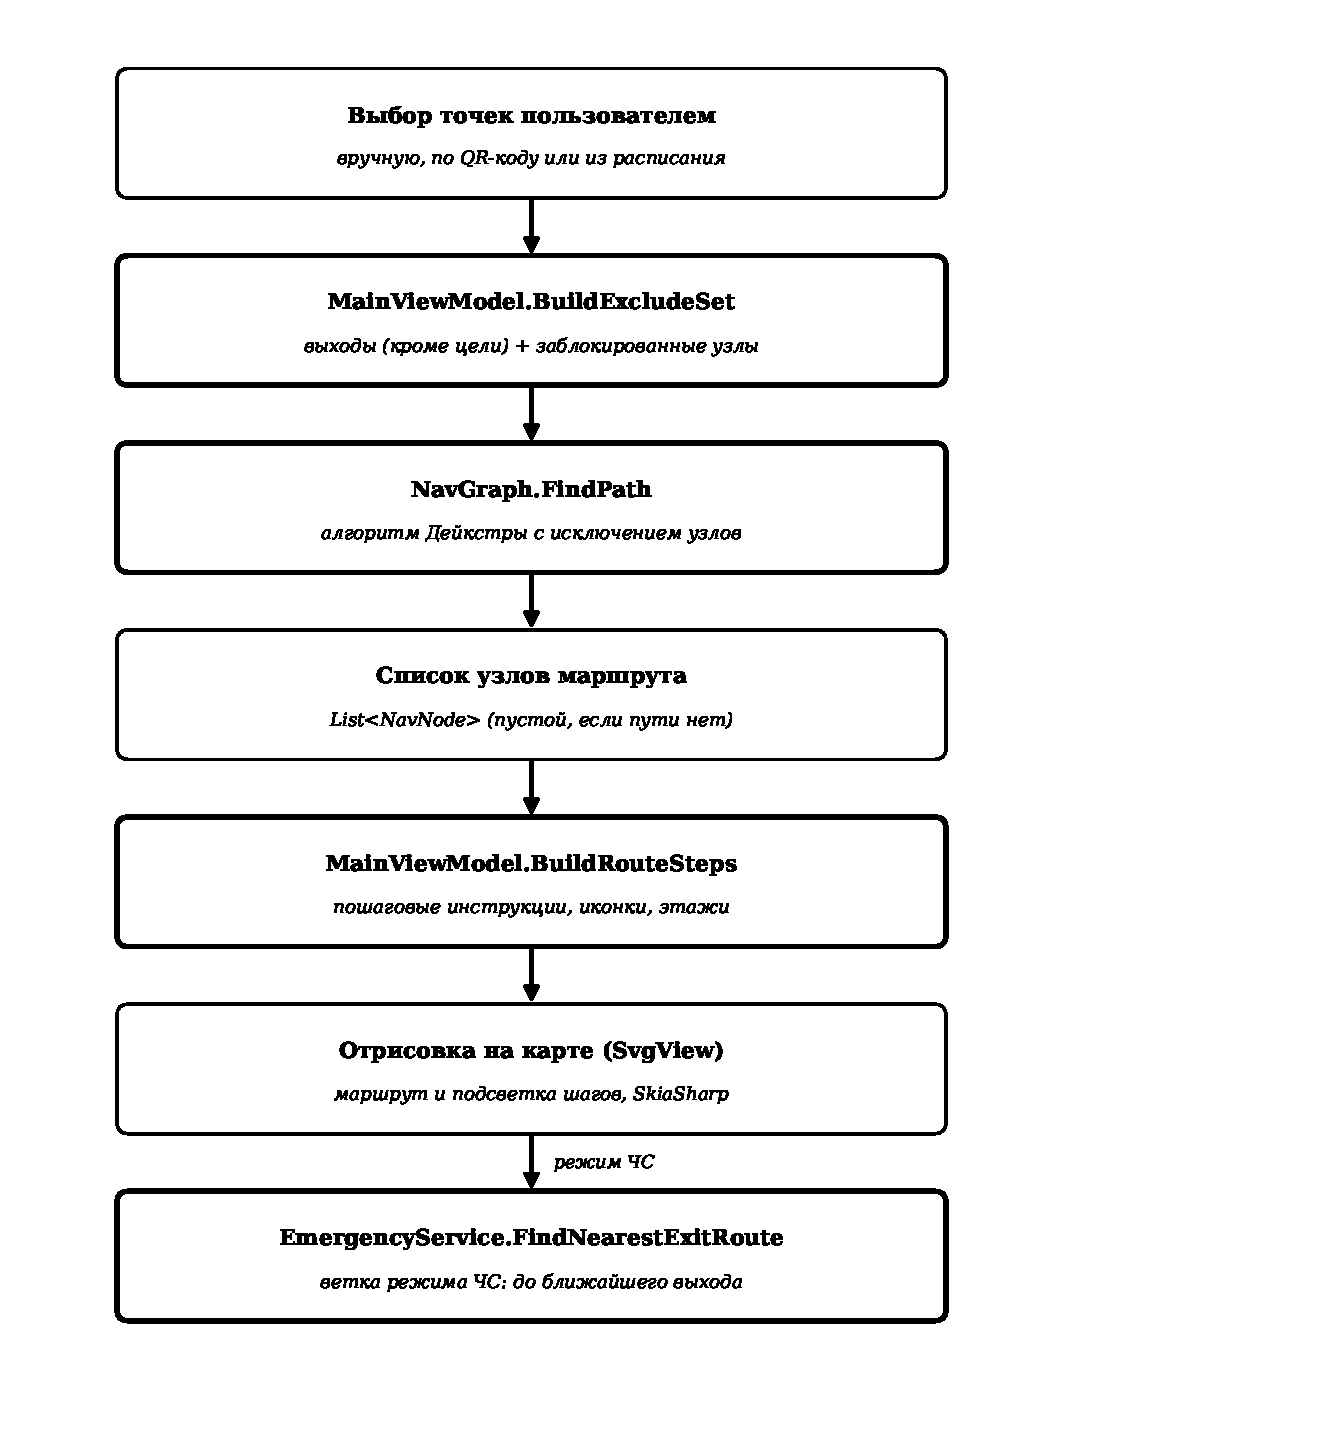
\includegraphics[width=0.7\textwidth]{Pictures/routeflow.eps}
	\caption{Процесс построения маршрута по слоям приложения}
	\label{routeflow:image}
\end{figure}

Сначала пользователь задаёт начальную и конечную точки~-- вручную, сканированием QR-кода или выбором аудитории из расписания. Затем \texttt{MainViewModel} собирает множество исключаемых узлов (\texttt{BuildExcludeSet}) и передаёт его вместе с концами маршрута в \texttt{NavGraph.FindPath}. Алгоритм Дейкстры возвращает список узлов; если он пуст, пользователю выводится сообщение о недоступности пути. Непустой маршрут уходит в \texttt{BuildRouteSteps}, который превращает его в пошаговые инструкции, после чего \texttt{SvgView} отрисовывает путь и подсвечивает текущий шаг на плане этажа.

В режиме ЧС поток выполнения отличается: вместо обычного построения маршрута вызывается \texttt{EmergencyService.FindNearestExitRoute}, который самостоятельно определяет ближайший выход, после чего обработка продолжается по той же цепочке (список узлов, инструкции, отрисовка). Единый поток выполнения позволяет обоим сценариям, повседневному и эвакуационному, использовать один и тот же код отображения.

\subsection{Проектирование пользовательского интерфейса}

Интерфейс проектировался по принципам человеко-ориентированного проектирования и удобства пользователя \cite{urbanovich2023,sterlyagov2017}: меньше действий до результата (маршрут строится не более чем в три касания), понятные подписи и адаптивная вёрстка под телефон и настольный компьютер. Разметка экранов описана на XAML, а данные связаны с моделями представления через привязку, поэтому одна и та же логика работает на всех платформах.

Приложение состоит из нескольких экранов:
\begin{enumerate}
	\item \textbf{Экран входа.} Гость заходит одним нажатием, студент~-- по логину и паролю. Роль определяет доступные дальше возможности.
	\item \textbf{Главный экран.} Занимает большую часть~-- интерактивный план этажа (контрол \texttt{SvgView} на SkiaSharp \cite{skiasharp}) с панорамированием и масштабированием. Сверху~-- поля <<Откуда>> и <<Куда>> с поиском по списку узлов и автодополнением по названию и тегам, кнопка построения маршрута и переключатель здания и этажа. После построения снизу появляются карточки пошаговых инструкций с кнопками <<Далее>>/<<Назад>> и счётчиком шагов; при ЧС сверху выводится предупреждающий баннер.
	\item \textbf{Экран QR-сканера.} Камера для считывания кода со стены (на Android и iOS); распознанный код задаёт начальную точку.
	\item \textbf{Панель администратора.} Редактор карты (добавление и соединение узлов, выбор их типа), управление пользователями и расписанием, включение режима ЧС по корпусам.
\end{enumerate}

Маршрут на плане выделяется отдельной линией с подсветкой текущего шага, а узлы-выходы и переходы между этажами обозначаются разными значками~-- чтобы пользователь различал их без подписей. Внешний вид главного экрана с построенным маршрутом приведён в разделе системного тестирования (рисунок~\ref{rproute:image}).

\subsection{Тестирование алгоритмов}

\textbf{Модульные тесты.} Разработан набор модульных тестов, покрывающих следующие сценарии: построение простого маршрута (линейный граф из 3 узлов), выбор оптимального пути при наличии альтернатив (разветвлённый граф), корректная работа на графе с циклами, обработка несуществующих идентификаторов узлов (возврат пустого списка), построение маршрута при исключении одного узла, полная блокировка пути (исключение всех промежуточных узлов, возврат пустого результата), поиск ближайшего выхода из нескольких вариантов, работа с одноузловым графом (старт = конец, возврат списка из одного элемента), маршрут с межэтажным переходом (проверка штрафного веса 150), последовательное исключение нескольких узлов, исключение конечного узла (должен быть достижим независимо от множества), пустой граф (нет узлов, возврат пустого списка), несвязный граф (старт и цель в разных компонентах связности).

\textbf{Тесты производительности.} Проведены замеры времени выполнения на тестовых данных различного объёма: граф с 50 узлами и 80 рёбрами -- среднее время 0,021 мс, граф с 200 узлами и 350 рёбрами -- 0,098 мс, граф с 500 узлами и 900 рёбрами -- 0,297 мс, поиск ближайшего выхода на графе 500 узлов -- 0,630 мс. Все замеры укладываются в требование $<200$ мс для построения маршрута и $<300$ мс для поиска выхода с многократным запасом. Результаты показывают линейный рост времени выполнения с увеличением размера графа, что согласуется с теоретической сложностью $O((V + E) \log V)$ для разреженных графов. Подробные результаты и график зависимости приведены в рабочем проекте (таблица~\ref{rpperf:table}).

\textbf{Интеграционные тесты.} Проведено тестирование с реальными данными навигационного графа здания университета: загрузка графа из \texttt{navgraph.json} и корректная десериализация, построение маршрутов между реальными аудиториями, корректность весов рёбер (совпадение с визуальным расстоянием на плане), поиск эвакуационного маршрута из различных стартовых точек, перестроение маршрута при блокировке реальных проходов.

\subsection{Сопоставление требований и компонентов}

Сопоставление требований, сформулированных в техническом задании, и компонентов их реализации приведено в таблице~\ref{algreq:table}.

\begin{xltabular}{\textwidth}{|X|X|}
\caption{Сопоставление требований и компонентов реализации\label{algreq:table}}\\ \hline
\centrow Требование & \centrow Компонент реализации \\ \hline
\endfirsthead
\continuecaption{Продолжение таблицы \ref{algreq:table}}
\centrow Требование & \centrow Компонент реализации \\ \hline
\finishhead
Поиск кратчайшего пути & \texttt{NavGraph.FindPath()} (алгоритм Дейкстры) \\ \hline
Динамическое исключение узлов & Параметр \texttt{excludeIds} в \texttt{FindPath} \\ \hline
Поиск ближайшего выхода & \texttt{EmergencyService.FindNearestExitRoute()} \\ \hline
Межэтажные переходы & Штрафной вес 150, флаг \texttt{IsCrossFloor} \\ \hline
Восстановление пути & Словарь \texttt{prev} + обратный обход \\ \hline
Структуры данных графа & \texttt{NavNode}, \texttt{NavEdge}, \texttt{NavGraph} \\ \hline
Сериализация & \texttt{System.Text.Json}, формат JSON \\ \hline
Пошаговые инструкции & \texttt{MainViewModel.BuildRouteSteps()} \\ \hline
Множество исключений & \texttt{MainViewModel.BuildExcludeSet()} \\ \hline
Производительность & \texttt{SortedSet}, \texttt{Dictionary}, список смежности
\end{xltabular}

\subsection{Выводы по о техническому проект}

В техническом проекте описана реализация алгоритмического ядра системы IndoorNav: выбор технологий (C\#, .NET, стандартные коллекции), структура модулей (NavNode, NavEdge, NavGraph, EmergencyService, NavGraphService), реализация алгоритма Дейкстры с поддержкой динамического исключения узлов, алгоритм поиска ближайшего эвакуационного выхода, механизм формирования пошаговых инструкций, формирование множества исключённых узлов, результаты модульного тестирования и замеров производительности, сериализация графа в JSON.

Разработанное алгоритмическое ядро обеспечивает эффективное построение эвакуационных маршрутов с учётом динамических препятствий. Использование алгоритма Дейкстры с современными структурами данных гарантирует производительность, соответствующую требованиям реального времени.
